\title{The Spectral Decomposition of a Symmetric Matrix}
\subtitle{\SubTitleName}
\institute[]{\Course}
\author{\Instructor}
\maketitle   
  


\frame{\frametitle{Topics and Objectives}
\Emph{Topics} \\
%\TopicStatement
\begin{itemize}

    % \item symmetric matrices
    % \item Orthogonal diagonalization
    \item the spectral decomposition of a matrix

\end{itemize}

\vspace{0.5cm}

\Emph{Learning Objectives}\\

%\LearningObjectiveStatement

\begin{itemize}

    % \item determine whether a matrix is symmetric
    % \item Construct an orthogonal diagonalization of a symmetric matrix, $A = PDP^T$. 
    \item construct a spectral decomposition of a matrix. 
    
\end{itemize}

\vspace{0.25cm} 


} 

\begin{frame}\frametitle{Motivation: Approximation}

    Recall that from calculus, Taylor expansions and Taylor polynomials, can be used to approximate functions near a point.
    \pause 
    \begin{center}
    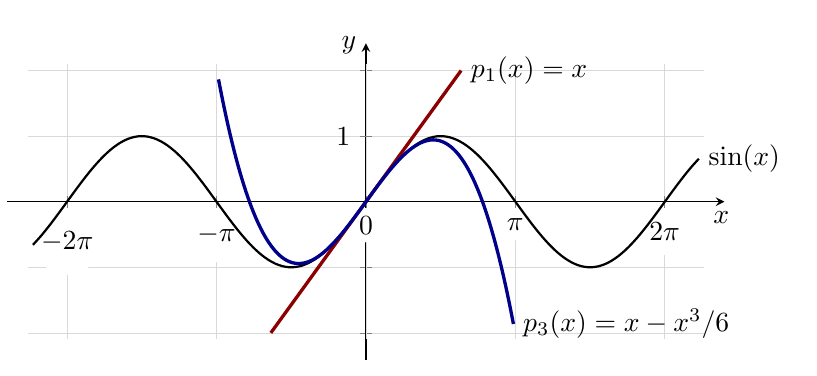
\begin{tikzpicture}[domain=-8:7] 
        \begin{axis}[
        width=4in,
        height=2.0in,
        grid=both,
        grid style={line width=.2pt, draw=gray!30},
        clip=false,
        axis lines=middle,
        xmin=-7.1,xmax=7.1,
        ymin=-2.1,ymax=2.1,
        restrict y to domain=-2:4,
        xtick={-6.28,-3.14,0,3.14,6.28},
        xticklabels={, , , , , , , , , ,},
        ytick={-2,-1,0,1,2},
        yticklabels={, , , , , , , , , ,},
        extra x ticks={-6.28,-3.14,0,3.14,6.28},
        extra y ticks={1},
        extra x tick style={xticklabel style={fill=white, circle, inner sep=1.5pt}},
        extra y tick style={xticklabel style={fill=white, circle, inner sep=1.5pt}},
        extra x tick labels={$-2\pi$, $-\pi$,$0$, $\pi$,$2\pi$},
        extra y tick labels={1},
        axis line style={shorten >=-7.5pt, shorten <=-7.5pt},
        xlabel=$x$,
        ylabel=$y$,
        xlabel style={at={(ticklabel* cs:1)},anchor=north west},
        ylabel style={at={(ticklabel* cs:1)},anchor=south east}
        ]
        
        \addplot[samples=100,domain=-7:7,smooth, thick] {sin(deg(x))} node[pos=1] (endofplotsquare) {};
        \node [right] at (endofplotsquare) {$\sin(x)$};  
        
        \addplot[samples=100,domain=-2:2,smooth, very thick,DarkRed] {x} node[pos=1] (endofplotsquare) {};
        \node [right] at (endofplotsquare) {$p_1(x)=x$};
        
        \addplot[samples=100,domain=-3.1:3.1,smooth, very thick,DarkBlue] {x-x*x*x/6} node[pos=1] (endofplotsquare) {};
        \node [right] at (endofplotsquare) {$p_3(x)=x-x^3/6$};           
        \end{axis}

    \end{tikzpicture}   
    \end{center}
    \pause Students are not expected to be familiar with Taylor expansions in this course, but, can we use expansions to approximate matrices? 
\end{frame}

\begin{frame}\frametitle{Motivation: Approximation}

    Can we use expansions to approximate matrices? \pause We will answer this question for two cases. 
    \pause 
    \begin{itemize}
        \item<2-> $A$ is a symmetric matrix (using an orthogonal diagonalization)
        \item<3-> $A$ is any real, $m\times n$ matrix (using the SVD)
    \end{itemize}
    \onslide<4->{We will introduce the SVD later in this course. For now, we will focus on the symmetric case. }
\end{frame}


\begin{frame}\frametitle{Spectral Decomposition of a Matrix}

    \begin{center}\begin{tikzpicture} \node [mybox](box){\begin{minipage}{0.75\textwidth}\vspace{4pt}
        Suppose $A$ can be orthogonally diagonalized as 
        \begin{equation*}
        A = P D P ^{T} = \begin{pmatrix}
        \vec u_1 & \cdots & \vec u_n 
        \end{pmatrix}
        \begin{pmatrix}
            \lambda _1 & \cdots & 0 
            \\
            \vdots & \ddots &  \vdots
            \\
            0 & \cdots & \lambda _n 
        \end{pmatrix}
        \begin{pmatrix}
            \vec u_1  ^{T}  \\ \vdots \\ \vec u_n  ^{T} 
        \end{pmatrix}
        \end{equation*}
        Then $A$ has the decomposition
        $$A = 
        \lambda _1 \vec u_1 \vec u_1 ^{T}  + \cdots + \lambda _n \vec u_n \vec u_n ^{T} 
        = \sum_{i=1}^{n} \lambda_i \vec u_i \vec u_i^T$$
        \end{minipage}};
    \node[fancytitle, right=10pt] at (box.north west) {Spectral Decomposition};
    \end{tikzpicture}\end{center}

    
\end{frame}


\begin{frame}\frametitle{Outline of the Spectral Decomposition Proof }    

    A short explanation on why $A$ has the decomposition
        $$A = 
        \lambda _1 \vec u_1 \vec u_1 ^{T}  + \cdots + \lambda _n \vec u_n \vec u_n ^{T} 
        = \sum_{i=1}^{n} \lambda_i \vec u_i \vec u_i^T$$

    \pause 
    We assume that we can write $A=PDP^T$. \pause If the columns of $D$ are $d_1,d_2, \ldots , d_n$, then, using the definition of matrix multiplication, 
    $$PD = \spalignmat{Pd_1 Pd_2 \ldots Pd_n}$$
    \pause 
    Then, what is $Pd_i$ equal to? 
\end{frame}


\begin{frame}\frametitle{Outline of the Spectral Decomposition Proof }    
    Recall that a matrix times a vector is a linear combination of the columns of the matrix weighted by the entries of the vector. \pause Column $i$ of $PD$ is 
    $$Pd_i = P\spalignmat{0;\vdots;0;\lambda_i;0;\vdots} = 0+0+\ldots +0 +\lambda_i \vec u_i+0 + \ldots =\lambda_i \vec u_i$$
    \pause Therefore, the columns of $PD$ are $\lambda_i \vec u_i$. We can now simplify our expression for $A=PDP^T$ to a product of two $n \times n$ matrices. 

\end{frame}


\begin{frame}\frametitle{Outline of the Spectral Decomposition Proof }        
    
    Thus, $A$ can be expressed as follows. 
    $$
    A = PDP^T = \begin{pmatrix}
        \lambda_1 \vec u_1 & \lambda_2 \vec u_2 & \cdots & \lambda_n \vec u_n 
        \end{pmatrix}
        \begin{pmatrix}
            \vec u_1  ^{T} \\ \vec u_2^T \\ \vdots \\ \vec u_n  ^{T} 
        \end{pmatrix}
    $$
    Using the \Emph{column-row expansion} for the product of two matrices, this becomes
    $$A = 
        \lambda _1 \vec u_1 \vec u_1 ^{T}  + \cdots + \lambda _n \vec u_n \vec u_n ^{T} 
        = \sum_{i=1}^{n} \lambda_i \vec u_i \vec u_i^T$$
    \textit{The row-column expansion for the product of two matrices is a way of defining matrix multiplication.}
\end{frame}


\begin{frame}\frametitle{Spectral Decomposition Example}

    Construct a spectral decomposition for $A$. 
    \begin{align*} 
        A = \spalignmat{3 1;1 3}
         &= 
         \spalignmat{1/\sqrt{2} -1/\sqrt{2}; 1/\sqrt{2} 1/\sqrt{2}}
         \spalignmat{4 0;0 2}
         \spalignmat{1/\sqrt{2} 1/\sqrt{2}; -1/\sqrt{2} 1/\sqrt{2}}
    \end{align*}
    \onslide<2->{\Emph{Solution}}
    \begin{align*}
        \onslide<2->{A &= \sum_{i=1}^2 \lambda_i \vec u_i \vec u_i\, ^T }\\
        \onslide<3->{&= 4 \spalignmat{1/\sqrt{2} ; 1/\sqrt{2}}\spalignmat{1/\sqrt{2} 1/\sqrt{2}} + 2  \spalignmat{-1/\sqrt{2} ; 1/\sqrt{2}}\spalignmat{-1/\sqrt{2} 1/\sqrt{2}} \\
        &= 4\spalignmat{0.5 0.5;0.5 0.5} + 2\spalignmat{0.5 -0.5;-0.5 0.5}}
    \end{align*}
    
    
    \end{frame}


\begin{frame}\frametitle{Spectral Decomposition Notes}

\begin{itemize}
    \item<1-> Each term in the sum $$\lambda_i\vec u_i \vec u_i^T$$ will be an $n \times n$ matrix with rank 1 (each column will be a multiple of $\vec u_i$). 
    \item<2-> Ordering the eigenvalues from largest to smallest (in absolute value),
    $$|\lambda_i | \ge |\lambda_{i+1}|$$
    we may be able to truncate the sum 
    $$A = \sum_{i=1}^{n} \lambda_i \vec u_i \vec u_i^T$$
    to exclude smaller terms. This gives us a way to approximate $A$. 

\end{itemize}
\end{frame}





\frame{\frametitle{Summary}

    \SummaryLine \vspace{4pt}
    \begin{itemize}\setlength{\itemsep}{8pt}

        \item spectral decomposition of a matrix: its definition and an example of its computation

    \end{itemize}
    
    \vspace{16pt}
    \pause 
    
}